\subsection{Implementación de un ABB mediante una estructura dinámica recursiva}
\begin{figure}[h]
  \begin{center}
    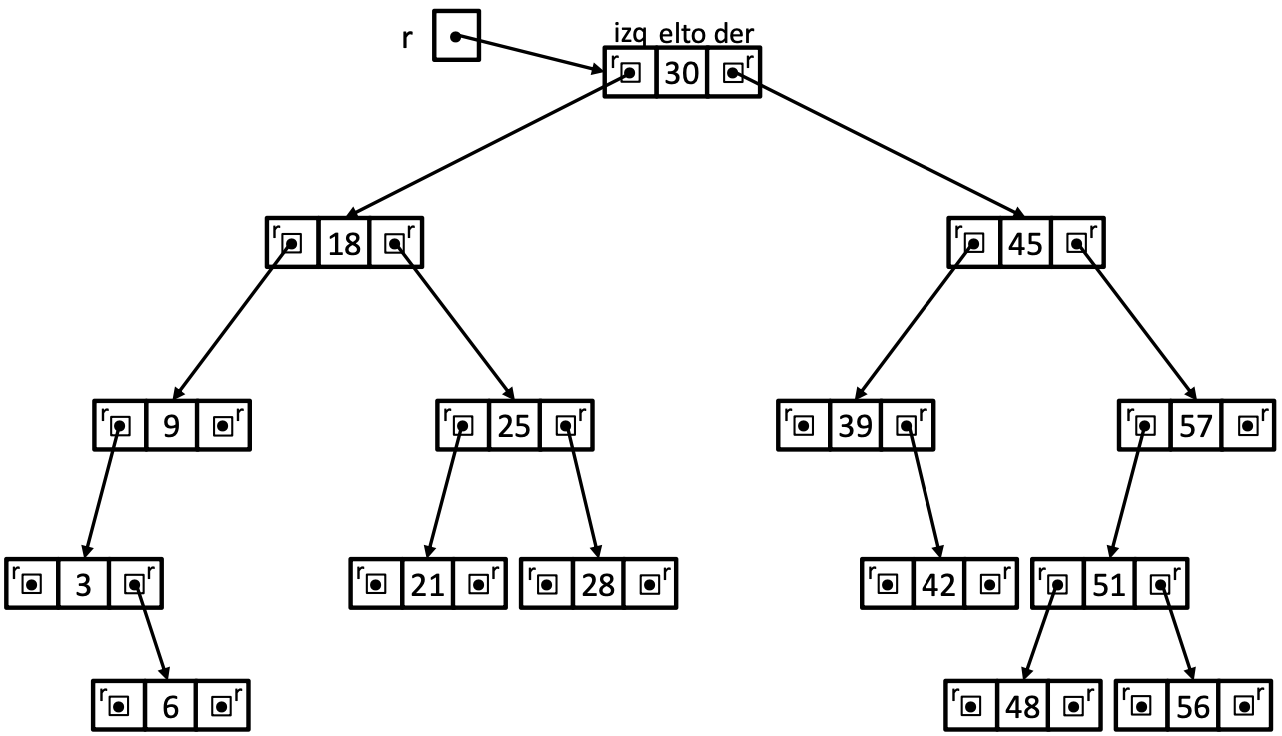
\includegraphics[width=0.6\textwidth]{assets/abb4.png}
  \end{center}
  \caption{Representación de la implementación dinámica recursiva}
\end{figure}

Vamos a hacer uso de esta implementación debido a que el método más `importante' de este TAD es el método \texttt{buscar()} (que nos devuelve el subárbol donde el elemento `e' es la raíz). Este método se realiza mediante llamadas recursiva y veremos como lo hace.

En la parte privada de TAD vamos a tener que almacenar el elemento y los dos subárboles (izquierdo y derecho).
\begin{minted}[breaklines]{C++}
template <typename T> class Abb{
  public:
    //Métodos vistos en la especificación del TAD
  private:
    struct arbol{
      T elto; //elemento
      Abb izq, der; //subárboles
      arbol(const T& e):elto(e),izq{},der{} {}
    };
    arbol *r;
};
\end{minted}
\subsubsection*{Implementación de la obtención del subárbol}
Ahora, vamos a ver como se implementa y que hace el método \texttt{buscar()}, mencionado anteriormente.
\begin{minted}[breaklines]{C++}
template <typename T>
const Abb<T>& Abb<T>::buscar(const T& e)const{
  if(r == nullptr)
    return *this; //Árbol vacio, no existe elemento
  else if(e < r->elto) //si es menor que el de la raiz, subárbol izquierdo
    return r->izq.buscar(e);
  else if(r->elto < e) //si es mayor, subárbol derecho
    return r->der.buscar(e);
  else 
    return *this; //encontrado en la raiz
}
\end{minted}

\subsubsection*{Inserción de un elemento en un ABB}
\begin{figure}[h]
  \begin{minipage}{0.4\textwidth}
    \vspace*{-2cm}
    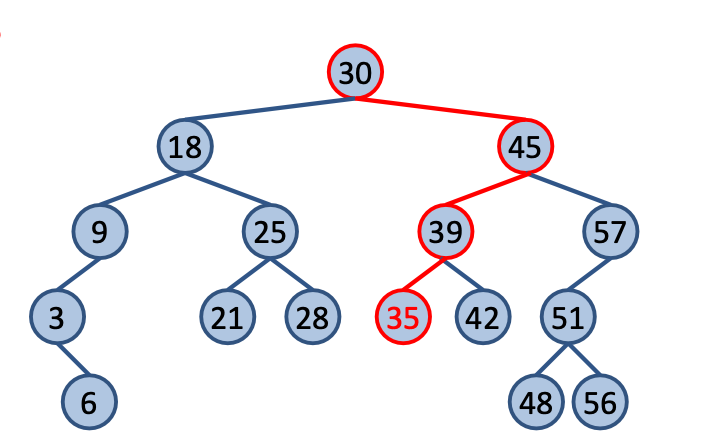
\includegraphics[width=\textwidth]{assets/abb5.png}
  \end{minipage}
  \hfill
  \begin{minipage}{0.5\textwidth}
    \begin{minted}[breaklines]{C++}
template <typename T>
void Abb<T>::insertar(const T& e){
  if(r==nullptr) //árbol vacio
      r = new arbol(e);
//se inserta en el subárbol izq.
  else if(e < r->elto) 
      r->izq.insertar(e);
//se inserta en el subárbol drch.
  else if(r->elto < e)
      r->der.insertar(e);
}
    \end{minted}
  \end{minipage}
\end{figure}

\underbar{\large\textbf{Ejemplo:}} Queremos insertar en el árbol anterior el elemento `35' (indicado en rojo),\\para ello la traza a seguir (según el código dado) sería:
\\
\hspace*{1cm}35 $>$ 30 → Hijo derecho de 30 → subárbol derecho.\\
\hspace*{1cm}35 $<$ 45 → Hijo izquierdo de 45 → subárbol izquierdo.\\
\hspace*{1cm}35 $<$ 39 → Hijo izquierdo de 39 → subárbol izquierdo.\\

Como el nodo cuyo valor es `39' no tiene subárbol izquierdo y 35 es menor que él, insertamos dicho valor como `hijo izquierdo' del nodo con valor 39.

\textit{NOTA}: Si encontramos que dicho valor ya se encuentra en el árbol no hacemos nada, ya que no podemos tener valores repetidos en el árbol.
\newpage
\subsubsection*{Eliminación de un elemento en un ABB}
A la hora de eliminar un elemento de un ABB no tenemos como precondición que el nodo que contiene a ese elemento sea una hoja, por tanto, encontramos 3 casos(cuando es hoja, tiene un hijo y tiene ambos hijos):

\begin{itemize}
  \item \textbf{Caso 1: Eliminación de un nodo hoja:}
  
    \begin{minipage}{0.4\textwidth}
      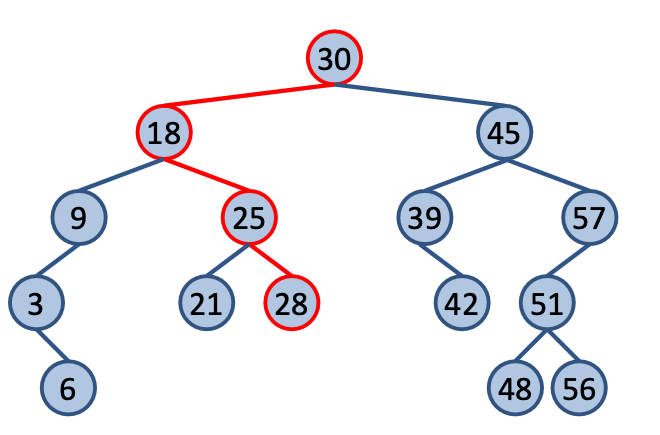
\includegraphics[width=\textwidth]{assets/abb6.png}
    \end{minipage}
    \hfill
    \begin{minipage}{0.5\textwidth}
    Queremos eliminar el nodo con elemento `28'(indicado en rojo), para ello:
    \\
    28 $<$ 30 → Hijo izquierdo de 30 → subárbol izquierdo.\\
    18 $<$ 28 → Hijo derecho de 18 → subárbol derecho.\\
    25 $<$ 28 → Hijo derecho de 25 → subárbol derecho.\\
    Como 28 = 28, lo eliminamos.
    \end{minipage}
    \underbar{Como resultado quedaría:}
  \begin{center}
    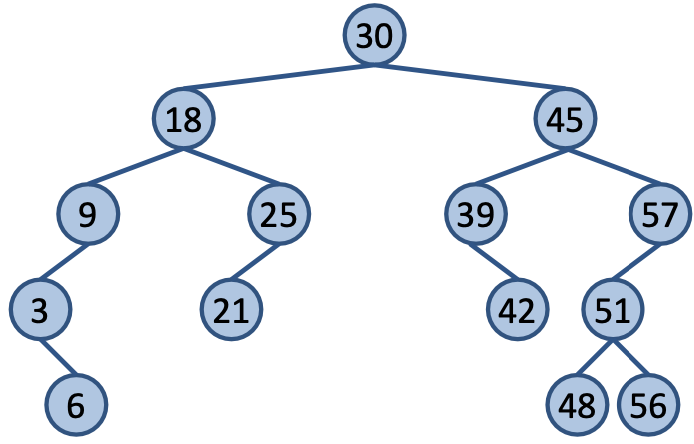
\includegraphics[width=.4\textwidth]{assets/abb11.png}
  \end{center}
  \item \textbf{Caso 2: Eliminación de un nodo con un hijo:}\\
  Este caso es un poco diferente, ya que el nodo a eliminar va a tener o hijo izquierdo o derecho.\\
  \begin{minipage}{0.4\textwidth}
    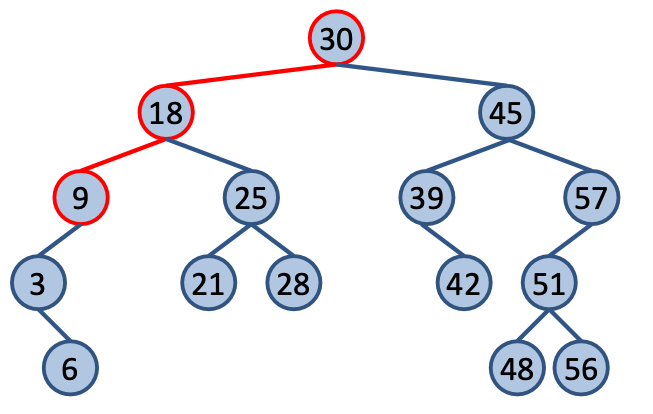
\includegraphics[width=\textwidth]{assets/abb7.png}
  \end{minipage}
  \hfill
  \begin{minipage}{0.5\textwidth}
  Queremos eliminar el nodo con elemento `9'(indicado en rojo), para ello:
  \\
  9 $<$ 30 → Hijo izquierdo de 30 → subárbol izquierdo.\\
  9 $<$ 18 → Hijo derecho de 18 → subárbol derecho.\\
  Como 9 = 9, lo eliminamos y su hijo pasa a ser el nuevo hijo izquierdo del `padre de 9', es decir el nodo con valor `18'.
  \end{minipage}

  \underbar{Como resultado quedaría:}
  \begin{center}
    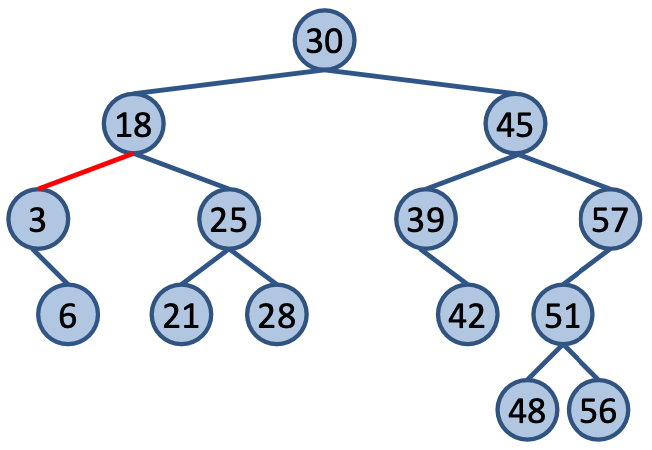
\includegraphics[width=.4\textwidth]{assets/abb10.png}
  \end{center}
  \newpage

  \item \textbf{Caso 3: Eliminación de un nodo con ambos hijos:}
  
  Este caso es parecido al caso 2, con la única diferencia que ahora el nodo a eliminar tiene tanto hijo izquierdo como derecho. Esto se soluciona buscando a los candidatos para ocupar su posición en el árbol, estos pueden ser el \textbf{mayor elemento del subárbol izquierdo} o el \textbf{menor elemento del subárbol derecho}.

  \begin{minipage}{0.4\textwidth}
    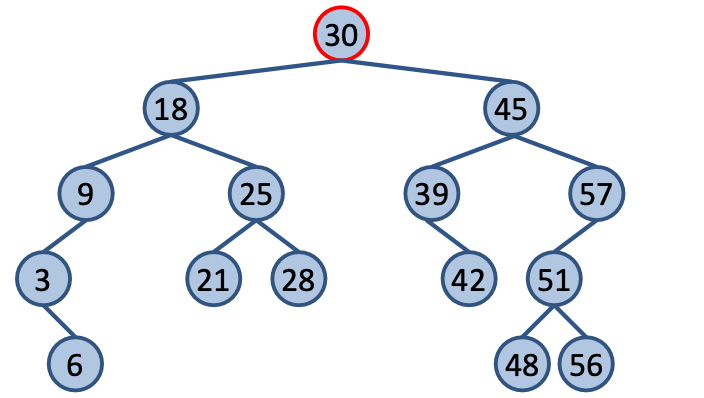
\includegraphics[width=\textwidth]{assets/abb8.png}
  \end{minipage}
  \hfill
  \begin{minipage}{0.5\textwidth}
  Como vemos, queremos eliminar el nodo con valor `30' (tiene dos hijos 18 y 45). Por tanto, los candidatos válidos son el nodo con mayor valor del subárbol que tiene como raíz `18' ó el nodo con menor valor del subárbol que tiene como raíz `45'.

  Hemos escogido el nodo con menor valor del subárbol derecho que es `39', pero este tiene un hijo derecho `42' que pasará a ser hijo izquierdo del nodo con valor `45'.
  \end{minipage}
  \underbar{Como resultado quedaría:}
  \begin{center}
    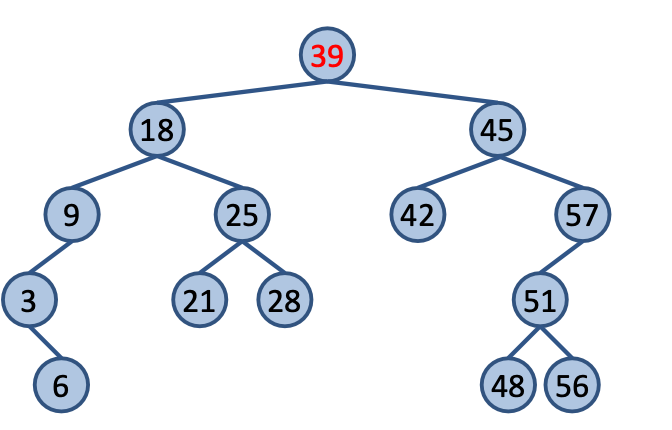
\includegraphics[width=.4\textwidth]{assets/abb9.png}
  \end{center}
\end{itemize}

\textbf{Código de la eliminación de elementos de un ABB:}
\begin{minted}[breaklines]{C++}
template <typename T> void Abb<T>::eliminar(const T& e){
  if(r!=nullptr){ //Caso 1: es hoja
    if(e < r->elto)
      r->izq.eliminar(e);
    else if(r->elto < e)
      r->der.eliminar(e);
  }
  else if(!r->izq.r && !r->der.r) //raíz es hoja
    delete r;
    r == nullptr;
  else if(!r->der.r) //Caso 2: Solo tiene un hijo (izquierdo)
    arbol *a = r->izq.r;
    r->izq.r = nullptr;
    delete r;
    r = a;
  else if(!r->izq.r) //Caso 2: Ánalogo para el derecho
    arbol *a = r->der.r;
    r->der.r = nullptr;
    delete r;
    r = a;
  else //Caso 3: Tiene ambos hijos
    r->elto = r->der.borrarMin();
}
\end{minted}
